% \glsresetall
\chapter{Micro frontend framework Luigi} % Main chapter title
\label{Chapter2}

\lhead{Chapter 2. \emph{Micro frontend framework Luigi}}

In this chapter, an overview of the used Luigi framework is given.

Currently there are different micro frontend frameworks available on the market, including but not limited to \textbf{Bit, SystemJS, Webpack 5 Module Federation, Piral, Single SPA} and \textbf{Luigi}.\cite{top10_mffs}
For the implementation of the representative landscapes the Luigi framework was used. Therefore, a short introduction to Luigi it is given here.

\section{Luigi}

Luigi is an open-source JavaScript framework for micro frontends, consisting of two main parts, the \textbf{Luigi Core} and the \textbf{Luigi Client}. It provides a basis to integrate micro frontends, also called \textbf{Nodes} in this context. Both parts serve different purposes in the micro frontend landscape.\cite{luigi_doc_overview}

\subsection{Core}

The \textbf{Luigi Core} is the basis of the whole landscape. It defines the main app, which will serve as an entry point for the user. The possibilities for, applicable configurations of this part are the following:

\begin{itemize}[noitemsep]
	\item Navigation - enables navigation between micro frontends
	\item Authorization - enables authorization for the landscape
	\item Localization - providing translations to display its applications in multiple languages
	\item General settings - e.g. header display configurations, enable loading indicators for the micro frontends, etc.
	\item Luigi Core API - providing functions for the core app to interact with the framework and access its features
\end{itemize} 

The core application inside the landscape is determined via the \texttt{luigi.config.js}. Any project containing it can fulfill this role, which is the only prerequisite. In the context of the framework, this app is later referred to as the \textbf{Core}.
Following this principle, the project structure of the \textbf{Core} could look as shown in listing \ref{list:luigi_core_structure}.\footnote{This example is taken directly from the implemented core project.}  

\begin{lstlisting}[language=Bash, caption=Project structure for a Luigi Core application including the \texttt{luigi.config.js}, label=list:luigi_core_structure,  xleftmargin=.0\textwidth, xrightmargin=.0\textwidth]
	- react-core-mf
		- [...]
		- node_modules
		- public
			- [...]
			- index.html
			- luigi.config.js
		- [...]
		- src
\end{lstlisting}

In the \texttt{luigi.config.js} itself the above mentioned possible configurations are defined.\cite{luigi_doc_core}

\subsection{Client}

The Luigi Client serves as the connection between the framework and its micro frontends. In order to establish the connection, a micro frontend has to import and initialize the Client. This will grant the micro frontend access to the \textbf{LuigiClient} object during the runtime. The micro frontend can then interact with the framework to e.g. set a global state, add event listeners or enable navigation between other micro frontends in the landscape.

An import of the Luigi Client can be accomplished via different methods. The most straightforward approach is the direct import with a HTML script tag. Another option would be the import of the local package manager dependency.\cite{luigi_client}

\begin{lstlisting}[caption=Import methods of the Luigi Client, label=list:import_luigi_client,  xleftmargin=.0\textwidth, xrightmargin=.0\textwidth]
	<!-- Via a HTML script tag -->
	<script src="https://unpkg.com/@luigi-project/client@1.17.0/luigi-client.js">
	</script>
	
	<!-- Via a package manager -->
	import LuigiClient from "@luigi-project/client";
\end{lstlisting}

\section{Architecture}

After the short introduction of the framework's core components, a general architecture of a landscape using Luigi is provided in figure \ref{fig:luigi_architecture_fig}.

\begin{figure}[!h]
	\centering
	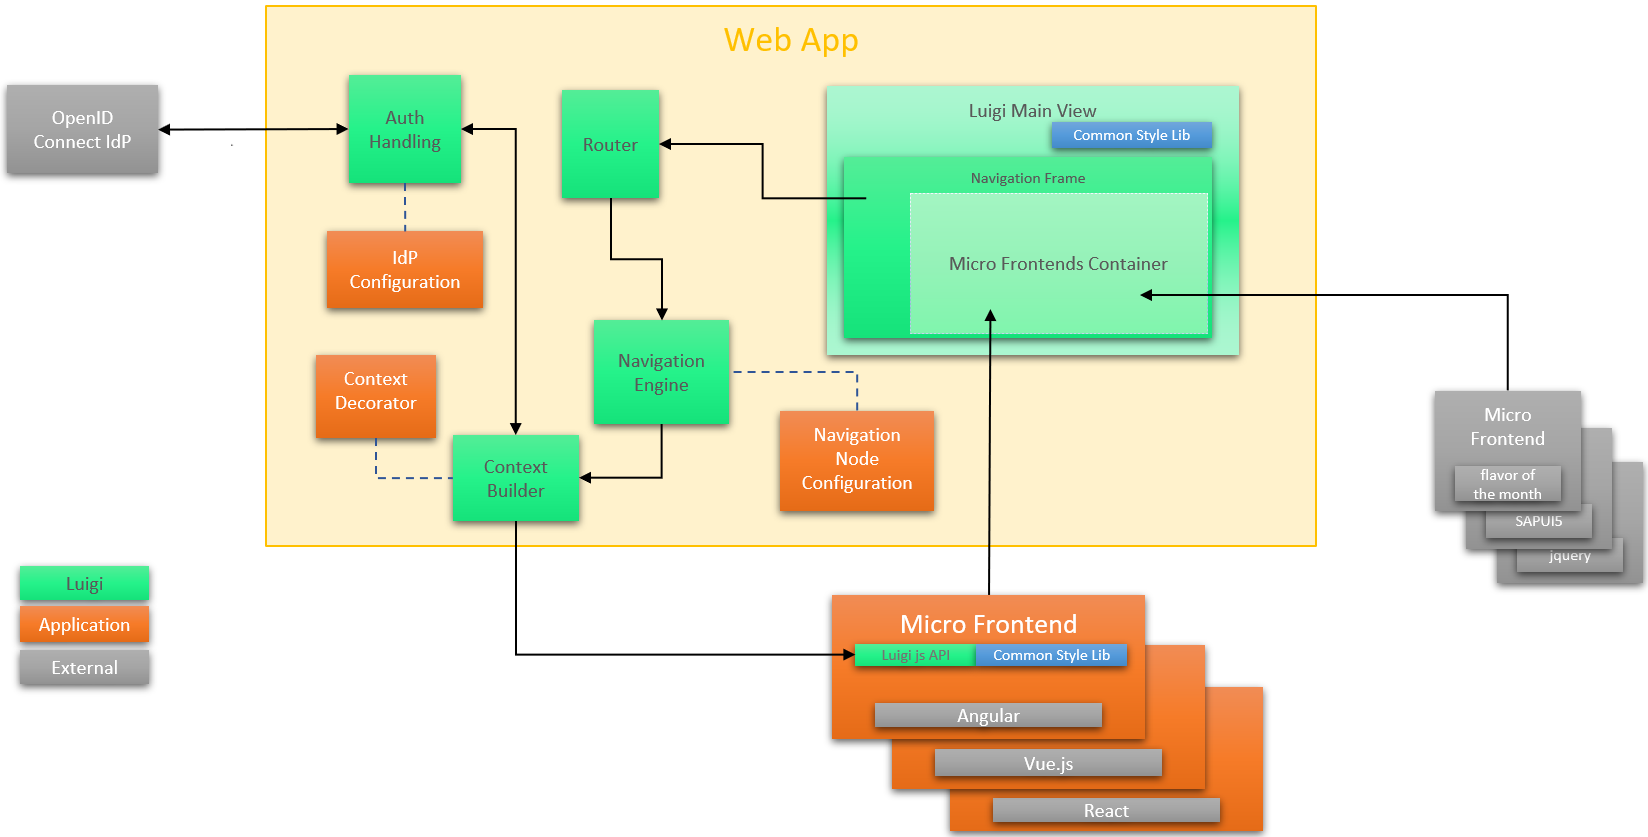
\includegraphics[width=1.05\textwidth]{Figures/Luigi_Architektur.png}
	\caption{Architecture of the Luigi Framework \cite{luigi_architecture}}
	\label{fig:luigi_architecture_fig}
\end{figure}

As can be seen in figure \ref{fig:luigi_architecture_fig}, the displayed micro frontends in the Web App have a distinguished position in the Micro Frontends Container. The embedded projects can either be integrated via iFrames or as Web Components.
Via the provided dashboard (Navigation Frame), the Luigi Core features are used. Through it, the navigation or search feature can be accessed.

As described in the first chapter of this transcript, the issue in such a landscape are the redundantly imported libraries of the embedded micro frontends. The reason for this problem is that each node is an isolated application.
For instance, navigating to the first micro frontend, followed by the second one, will load the bundled projects with their corresponding dependencies. In this case, the browser has no way to distinguish if a loaded resource is already present or not. The reason for that is the bundling of projects which makes the references indistinguishable to the browser.
The following chapters will introduce technologies, which offer methods to resolve this issue. 
 
